\documentclass[conference]{IEEEtran}

\usepackage{amsmath}
\usepackage{amssymb}
\usepackage{graphicx}
\usepackage{booktabs}
\usepackage{multirow}
\usepackage{hyperref}
\usepackage{cite}
\usepackage{listings}
\usepackage{xcolor}
\usepackage{underscore}

\lstset{
  basicstyle=\ttfamily\footnotesize,
  breaklines=true,
  columns=fullflexible,
  frame=single,
  showstringspaces=false,
  language=C++
}

\newcommand{\rclcpp}{\texttt{rclcpp}}

\begin{document}

\title{STRATA: One Geometry-Free Persistence-and-Periodicity Engine\\
Driving Selectable 2D/3D Lifelong LiDAR Mapping in ROS~2}

\author{
  \IEEEauthorblockN{Jungmo Kang}
  \IEEEauthorblockA{Independent Researcher\\
  kangjmo91@gmail.com\\
  \url{https://github.com/kjungmo}}
}

\maketitle

\begin{abstract}
A robot that maps the same building for weeks cannot bake every LiDAR hit
permanently into one grid: parked carts, passing people, and doors that open on
a schedule all burn in, and the map slowly ossifies into a record of everything
that was ever seen rather than of what is actually there now. Lifelong mapping
must instead hold three properties in tension at once --- durability (keep the
walls), plasticity (forget the movers), and periodicity (treat a cyclic door as
signal, not noise). We present STRATA, a small, geometry-free
persistence-and-periodicity engine that resolves this tension in one shared
per-cell state machine and drives two pluggable geometry backends --- a
fixed-array 2D occupancy grid and an unbounded 3D voxel-hash --- behind a single
interface selected by one runtime string parameter. The only per-backend code
is point-to-id mapping and the free-space ray walk; the classifier that
graduates, demotes, prunes, and periodicity-labels every cell is shared by
composition, not duplicated per dimension. The engine is a plain C++17 + Eigen
library with no ROS, DDS, or PCL dependency, exercised by 22 behavior-level
tests, so its scientific logic builds and runs deterministically in a
second-scale CI loop. A seeded synthetic characterization suite reports that
both backends graduate a static wall by the third window and hold recall 1.0
thereafter (their only divergence, a clutter-induced static-precision gap of
0.9253 vs.\ 0.9758 under 100 movers per window, is geometric, not algorithmic);
that 50\%-duty periodic doors are detected at true-positive rate 2/3 and
false-positive rate 1/5; that removing hysteresis inflates flicker from 54 to
574 toggles on identical replayed noise (at fixed decay $\lambda=0.90$); and that the unified engine costs a
flat $\sim$56~B per cell with no per-dimension penalty. Evaluation is synthetic and
the tool performs no SLAM; STRATA is the persistence core meant to sit beneath
an external localizer, released open-source as a ROS~2 package.
\end{abstract}

\begin{IEEEkeywords}
lifelong mapping, occupancy grids, voxel mapping, persistence filtering, FreMEn periodicity, ROS~2, open-source robotics software
\end{IEEEkeywords}

\section{Introduction}

An occupancy grid built the textbook way accumulates evidence and never lets go
of it. For a robot that drives a route once, that is fine. For one that maps the
same warehouse or hospital corridor for weeks, it is a slow failure: every hit
is folded into the same static belief, so a cart parked for an afternoon, a
person walking past, and a load-bearing wall all leave the same kind of mark.
Over enough passes the map stops describing the building and starts describing
the union of everything the sensor ever touched. Suppressing that failure is the
whole problem of lifelong mapping, and it forces three requirements that pull in
different directions: the map must be \emph{durable} enough to keep structure that is
genuinely permanent, \emph{plastic} enough to forget structure that has moved on, and
must do both without a single global forgetting rate that is simultaneously too
slow to erase movers and too fast to trust a wall. This is the
stability--plasticity dilemma that Biber and Duckett framed for dynamic maps
\cite{biber2005dynamicmaps}: represent the environment at more than one timescale at
once, or lose either the walls or the ability to adapt.

A third requirement complicates the split further. Some structure is neither
permanent nor transient but \emph{cyclic} --- a door open every morning and shut every
night, a shutter that tracks business hours. Krajn\'ik et al.\ show that such a
cell's occupancy is a periodic temporal signal, and that a flat decay law
erases exactly the regularity that makes it predictable, discarding information
a robot could have exploited \cite{krajnik2017fremen,krajnik2014spectral}. A
lifelong map therefore needs three coexisting timescales, not two: a fast-fading
occupancy signal, a slowly-graduated durable class, and a separately-timed
periodic class that a decay term alone would flatten into noise.

The systems that come closest to solving this are heavier than the problem needs
to be. ELite \cite{gil2025elite} and LT-mapper \cite{kim2022ltmapper} --- the closest
published twins in intent --- resolve durability versus plasticity, but as parts
of full lifelong-\textbf{SLAM} pipelines, coupled to multi-session point-cloud
registration, place recognition, and alignment. RTAB-Map \cite{labbe2019rtabmap} is
the closest engineering precedent for offering selectable 2D and 3D geometry
under one framework, but it too is a complete SLAM system with loop closure and
memory tiering. Each carries the persistence-and-classification logic a robot
needs, but welded inside a much larger apparatus and to a specific map
geometry. What is missing from the surveyed prior art is the small piece by
itself: a standalone, SLAM-free, dependency-light engine that does only the
graduation, forgetting, and periodicity classification, that runs under either
2D or 3D geometry, and that a practitioner can drop beneath an external
localizer or an existing SLAM front end.

STRATA is that piece. The name is literal: a cell in the map carries temporal
strata --- Static, Periodic, and Transient layers over an Unknown baseline ---
coexisting inside one per-cell state machine, read and written by log-odds
occupancy, survival decay, Schmitt-trigger hysteresis, and an incremental
Fourier periodicity test. That state machine is geometry-free. Both shipped
backends translate world points into \texttt{int64} cell keys and walk a free-space
ray to clear it; everything downstream of the key --- accumulation, graduation,
demotion, pruning, periodicity labeling --- happens once, in the shared engine.
The thesis is deliberately narrow: \emph{the only per-backend code is point-to-id
mapping and the free-space ray walk; the classifier is shared by composition,
not duplicated per dimension} (Fig.~\ref{fig:architecture}). Selecting 2D versus 3D is a single
runtime string parameter resolved at construction, not a plugin-loading
mechanism, and the engine itself (\texttt{strata\_core}) is a plain C++17 + Eigen
library with no \texttt{rclcpp}, \texttt{tf2}, PCL, or DDS dependency, so its scientific logic
builds and unit-tests without a ROS install.

We are explicit about scope up front (\S\ref{sec:discussion} consolidates the non-claims). STRATA is
\textbf{not SLAM}: it estimates no pose, closes no loops, and aligns no sessions,
consuming instead an external \texttt{map} $\to$ \texttt{sensor} transform. Its evaluation is
\textbf{synthetic only} --- every number below comes from deterministic seeded
harnesses and unit tests, not a field deployment, in contrast to the multi-day
validations of ELite, LT-mapper, and Berrio et al.\ \cite{berrio2021longterm}. And it
models \textbf{single-session} temporal persistence, not multi-session remapping: a
graduated cell simply \emph{is} the current static map, with no session versioning.
These are the boundaries of the tool, stated as scope rather than buried as
gaps.

\textbf{Contributions.} This paper makes five, each backed only by the shipped code
and the synthetic suite:

\begin{enumerate}
\item \textbf{One geometry-free engine, two geometries, one switch (by construction).}
   A single \texttt{int64}-keyed persistence-and-periodicity engine (\texttt{LayeredMap} +
   \texttt{PeriodicityModel}) drives both a fixed-array 2D occupancy grid and an
   unbounded 3D voxel-hash behind one \texttt{MapBackend} interface, chosen by a single
   runtime string parameter, with no state-machine logic duplicated across
   dimensions (Fig.~\ref{fig:architecture}; \S\ref{sec:system}--\ref{sec:method}).
\item \textbf{A ROS-free, deterministically testable core, shown backend-equivalent
   (design goal + measured).} The engine builds and unit-tests with a plain
   C++17 + Eigen toolchain and is exercised by 22 behavior-level tests; both
   backends graduate the static wall by window 3 and hold recall 1.0 through
   window 39, differing in static-layer quality only by a clutter-induced
   static-precision gap (0.9253 grid2d vs.\ 0.9758 voxel3d at 100 movers per
   window) that traces to 2D $z$-collapse geometry, not to the classifier; a
   separate per-\texttt{integrate()} cost gap between the backends is characterized in
   contribution 5 (\S\ref{sec:system}, \S\ref{sec:eval}).
\item \textbf{A specific minimal combination not previously packaged standalone.}
   Persistence-Filter survival decay \cite{rosen2016persistence}, Removert-motivated
   Schmitt hysteresis \cite{kim2020removert}, ReFusion-style negative-evidence ray
   clearing \cite{palazzolo2019refusion}, and a parallel FreMEn-lite periodicity
   classifier \cite{krajnik2017fremen}, emitting a four-class label from one
   dependency-light, SLAM-free module --- a combination absent, in this form, from
   the surveyed prior art (\S\ref{sec:related}, \S\ref{sec:method}).
\item \textbf{A mechanistic characterization of the shared classifier (measured).}
   50\%-duty periodicity is detected cleanly (dominant-harmonic amplitude
   0.653/0.707, well above the 0.3 threshold) at true-positive rate 2/3 and
   false-positive rate 1/5, with the single miss diagnosed as a prune/maturity
   race; and hysteresis is the dominant stabilizer --- removing it yields 574
   flicker toggles at F1 0.810 versus 54 toggles at F1 1.000 on identical
   replayed noise at the same decay ($\lambda=0.90$) (\S\ref{sec:eval}).
\item \textbf{A unified engine that adds no per-dimension cost, released as a
   reproducible tool (measured).} Memory is a flat $\sim$56~B per cell and
   per-window cost tracks live-cell count linearly; the 5.5--14.9$\times$ per-\texttt{integrate()}
   gap between backends is entirely 3D free-space voxel proliferation (4.4--10.0$\times$
   more live cells), geometry rather than the engine. The whole system ships as
   an open-source ROS~2 package with a documented I/O contract and a seeded
   harness whose figures regenerate from measured CSVs (\S\ref{sec:system}, \S\ref{sec:eval}).
\end{enumerate}

STRATA is available at \texttt{github.com/kjungmo/strata} as a ROS~2 Humble package
under an open-source license, with a thin ROS adapter node and a reusable
characterization harness; it is designed to plug beneath an external localizer
such as \texttt{prism\_loc}. The remainder of the paper positions STRATA against the
prior art (\S\ref{sec:related}), specifies its two-band, testable architecture (\S\ref{sec:system}), gives the
as-shipped engine mathematics including three honest implementation-versus-
specification differences (\S\ref{sec:method}), reports the synthetic evaluation (\S\ref{sec:eval}), and
states the limitations, boundaries, and reproducibility of the tool (\S\ref{sec:discussion}--\S\ref{sec:conclusion}).

\section{Related Work}
\label{sec:related}

We organize prior work into six themes and, for each entry, state STRATA's
exact relation rather than a generic contrast.

\textbf{Lifelong and persistent mapping.} ELite \cite{gil2025elite} and LT-mapper
\cite{kim2022ltmapper} are STRATA's closest published twins. ELite computes a
two-timescale ephemerality score per point (within-session dynamic vs.\
across-session transient) and drives a Lifelong/Static/Delta map triad;
LT-mapper composes a live map, a meta map, and a delta map through explicit
LT-SLAM alignment, LT-removert removal, and LT-map graduation stages. Both
are full lifelong-SLAM pipelines with multi-session point-cloud registration
and place recognition. STRATA implements only the graduation half of that
pattern --- one per-cell state machine (Static/Periodic/Transient/Unknown,
\S\ref{sec:states}) inside a ROS-free engine, with no scan matching, no loop closure, and
no cross-session alignment. STRATA is not a competing full system; it is the
persistence-and-classification core that ELite's triad and LT-mapper's
live-to-static pipeline wrap around, and its measured evaluation (\S\ref{sec:eval}) is
correspondingly narrower --- a synthetic, single-session characterization, not
the field-scale validation ELite and LT-mapper report. Khronos
\cite{schmid2024khronos} generalizes the same two-timescale idea to an
active-window/long-term-reconstruction split with semantics and a scene
graph; STRATA stays at the raw per-cell level with no object or scene-graph
layer, a narrower and cheaper instance of the same principle. Biber and
Duckett \cite{biber2005dynamicmaps} and Meyer-Delius et al.\
\cite{meyerdelius2010temporary} are the foundational multi-timescale and
static/temporary-split ideas STRATA's window/decay/hysteresis/periodicity
combination descends from. RTAB-Map \cite{labbe2019rtabmap} is the closest
engineering precedent for selectable 2D/3D geometry inside one shipped
framework, coupled to full SLAM and STM/WM/LTM memory management; STRATA
narrows this to the mapping/persistence layer alone, behind a \texttt{MapBackend}
interface selected by a single string parameter, consuming an externally
supplied pose rather than estimating one. Berrio et al.\ \cite{berrio2021longterm}
report an 18-month field deployment of the same purge/promote pattern STRATA
implements as a Schmitt trigger (\S\ref{sec:schmitt}) --- field-scale evidence for the pattern
that STRATA currently lacks for itself. Yang et al.\ \cite{yang2025lifelong3d}
keep positive/negative version deltas over a base map so any past session can
be reconstructed; STRATA does no session versioning at all --- a graduated cell
is simply part of the current static map, its history implicit in log-odds
and observation counts, not explicitly replayable.

\textbf{Persistence and forgetting.} The Persistence Filter \cite{rosen2016persistence}
recursively estimates each feature's survival probability from a Bayesian
survival-time model. STRATA's per-window survival-decay multiplier $\lambda$
(\S\ref{sec:logodds}) is a discretized, single-scalar simplification of that idea: one tunable
multiplicative factor pulls belief toward unknown each window in place of a
full survival-time posterior. The log-odds hit/miss update with clamping in
Thrun et al.\ \cite{thrun2005probabilistic} is used verbatim as STRATA's per-window
occupancy accumulation, with decay and hysteresis layered on top. Tipaldi et
al.\ \cite{tipaldi2013lifelong} and Saarinen et al.\ (iMac) \cite{saarinen2012imac}
model each cell as a two-state Markov process with a recency-weighted or
online-learned transition rate --- the principled, per-cell-learned form of
"how fast a cell should forget." \texttt{survival\_decay} is a single global
constant, a constant-rate special case of that formalism; STRATA states this
as a documented simplification (\S\ref{sec:discussion}), not an unacknowledged gap.

\textbf{Periodicity.} FreMEn \cite{krajnik2017fremen} is the direct counter-argument
STRATA's Periodic class answers: a cell's occupancy can be a periodic
temporal signal, and a flat decay erases exactly that structure. STRATA's
\texttt{PeriodicityModel} (\S\ref{sec:periodicity}) runs FreMEn's incremental-Fourier accumulation in
parallel with decay and graduation, so an oscillating cell is classified
Periodic rather than mis-graduated to Static or mis-pruned as Transient --- the
third class exists specifically to answer this argument, at the cost of a
bounded harmonic count and a validity gate tied to touched-window count
rather than elapsed time (a documented implementation-versus-specification
divergence, \S\ref{sec:specdiff}). Krajn\'ik et al.\
\cite{krajnik2014spectral} is the earlier, more general spectral-analysis
lineage FreMEn later packaged as a mapping method; STRATA's bounded
incremental-Fourier approximation is a further narrowing of that lineage, not
the full spectral machinery.

\textbf{Dynamic-object removal.} Removert \cite{kim2020removert} conservatively
removes dynamic points and then reverts wrongly removed static ones, because
aggressive removal erases real structure. This is the exact justification for
STRATA's hysteresis band (\S\ref{sec:schmitt}): a graduated cell demotes only when its
probability falls below $p_{\text{dem}} < p_{\text{grad}}$, i.e.\ sustained contradicting
evidence across windows rather than a single contradicting frame --- the same
failure mode Removert's revert pass patches after the fact, STRATA prevents
online by construction. ReFusion \cite{palazzolo2019refusion} treats a reliably
observed empty voxel as evidence, not merely an absence of evidence; STRATA's
ray-clearing --- exact Bresenham for \texttt{grid2d}, sub-voxel-step sampling for
\texttt{voxel3d} (\S\ref{sec:backends}) --- applies the same negative-information logic online, with
misses accumulating as $l_{\text{miss}}$ and eventually demoting a graduated cell once
an object vacates it. ERASOR \cite{lim2021erasor} removes dynamic points from an
already-accumulated 3D map offline via per-bin pseudo-occupancy ratios; STRATA
never batches and performs no object-level reasoning --- every cell's class is
a running online per-window hit/miss-and-decay state, the baseline ERASOR's
batch, object-level approach is not attempting to be.

\textbf{Production stacks.} OctoMap \cite{hornung2013octomap} shares STRATA's
log-odds-with-clamping core but compresses storage with an octree; \texttt{voxel3d}
instead uses a flat \texttt{int64}-keyed hash for O(1) insert/lookup, trading
multi-resolution compression for simplicity and unit-testability (\S\ref{sec:discussion}). The
voxel-hashing scheme of Nie{\ss}ner et al.\ \cite{niessner2013hashing} is the direct
data-structure this hash follows. UFOMap \cite{duberg2020ufomap} makes "never
observed" an explicit third per-voxel state; STRATA gets the same distinction
implicitly from the \texttt{observations} counter and log-odds value rather than a
dedicated state, cheaper to implement and less explicit to query. Nav2 STVL
\cite{macenski2020stvl} decays costmap obstacle evidence for short-horizon
planning using the same decay-rate mechanism family STRATA's
\texttt{survival\_decay} uses to decay mapping evidence toward unknown --- same knob,
different consumer. Layered Costmaps \cite{lu2014layered} composite independently
maintained plugin layers per cell; STRATA's output value convention
(\texttt{static}$\to$100, \texttt{periodic}$\to$75, \texttt{transient}$\to$50, \texttt{unknown}$\to{-}1$)
reproduces the same
layered mental model as the output of one cell-level state machine rather
than as multiple composited layers. SLAM Toolbox \cite{macenski2021slamtoolbox}
bounds compute by adding and removing pose-graph nodes while performing its
own 2D SLAM; STRATA has no pose graph and no SLAM, consuming an externally
supplied transform and pruning at the per-cell evidence level (\S\ref{sec:states}) instead
--- a different layer of the stack, included as the standard 2D lifelong-mapping
comparison point.

\textbf{Pluggable-backend architecture.} ROS~2 Pluginlib \cite{ros2pluginlib} is the
canonical swappable-backend mechanism --- abstract base class, XML plugin
description, runtime \texttt{dlopen}-based loading --- and the pattern STRATA
deliberately rejects, not adopts. With exactly two backends, STRATA resolves
\texttt{MapBackend} to one of two \texttt{unique\_ptr}s at construction from a single
runtime string parameter (\S\ref{sec:system}); no plugin XML, no dynamic loading, no
\texttt{ament\_index} registry. This is the right choice at two backends; pluginlib
becomes the right choice only once backend count grows past what a single
\texttt{if}/\texttt{else} factory reads clearly. RTAB-Map \cite{labbe2019rtabmap} is re-cited
here as the closest existing shipped system offering selectable 2D/3D
geometry under one framework, narrowed by STRATA to a persistence-only
module with the classifier shared by composition rather than duplicated per
geometry --- the only per-backend code is point-to-\texttt{CellId} mapping and the
free-space ray walk.

None of the surveyed prior art offers, as a standalone, SLAM-free,
dependency-light module, the specific combination STRATA ships: survival
decay, Schmitt-trigger hysteresis, negative-evidence ray clearing, and
parallel FreMEn-lite periodicity classification, unified behind one
geometry-free engine and selectable between two map geometries at runtime.

\section{System Overview and Architecture}
\label{sec:system}

STRATA is delivered as two ament packages with a deliberate dependency
boundary between them. \texttt{strata\_core} is the scientific engine: pure C++17 with
Eigen as its only third-party dependency, holding the entire
occupancy/persistence/periodicity state machine and both geometry backends.
\texttt{strata} is a thin ROS~2 node that wraps the engine, owning message
conversion, TF lookups, publishers, subscribers, services, and file I/O. Every
ROS-only dependency --- \texttt{rclcpp}, \texttt{tf2}, \texttt{sensor\_msgs}, \texttt{nav\_msgs}, PCL --- lives
exclusively in \texttt{strata}; \texttt{strata\_core} links none of them. This split is the
reason the engine builds and unit-tests with a plain system toolchain
(\texttt{cmake -S strata\_core -B build -DSTRATA\_CORE\_BUILD\_TESTS=ON \&\& ctest}), with
no ROS install, no colcon, no DDS discovery, and no TF buffer warm-up in the
loop. The architecture is shown in Fig.~\ref{fig:architecture}.

\begin{figure}[t]
\centering
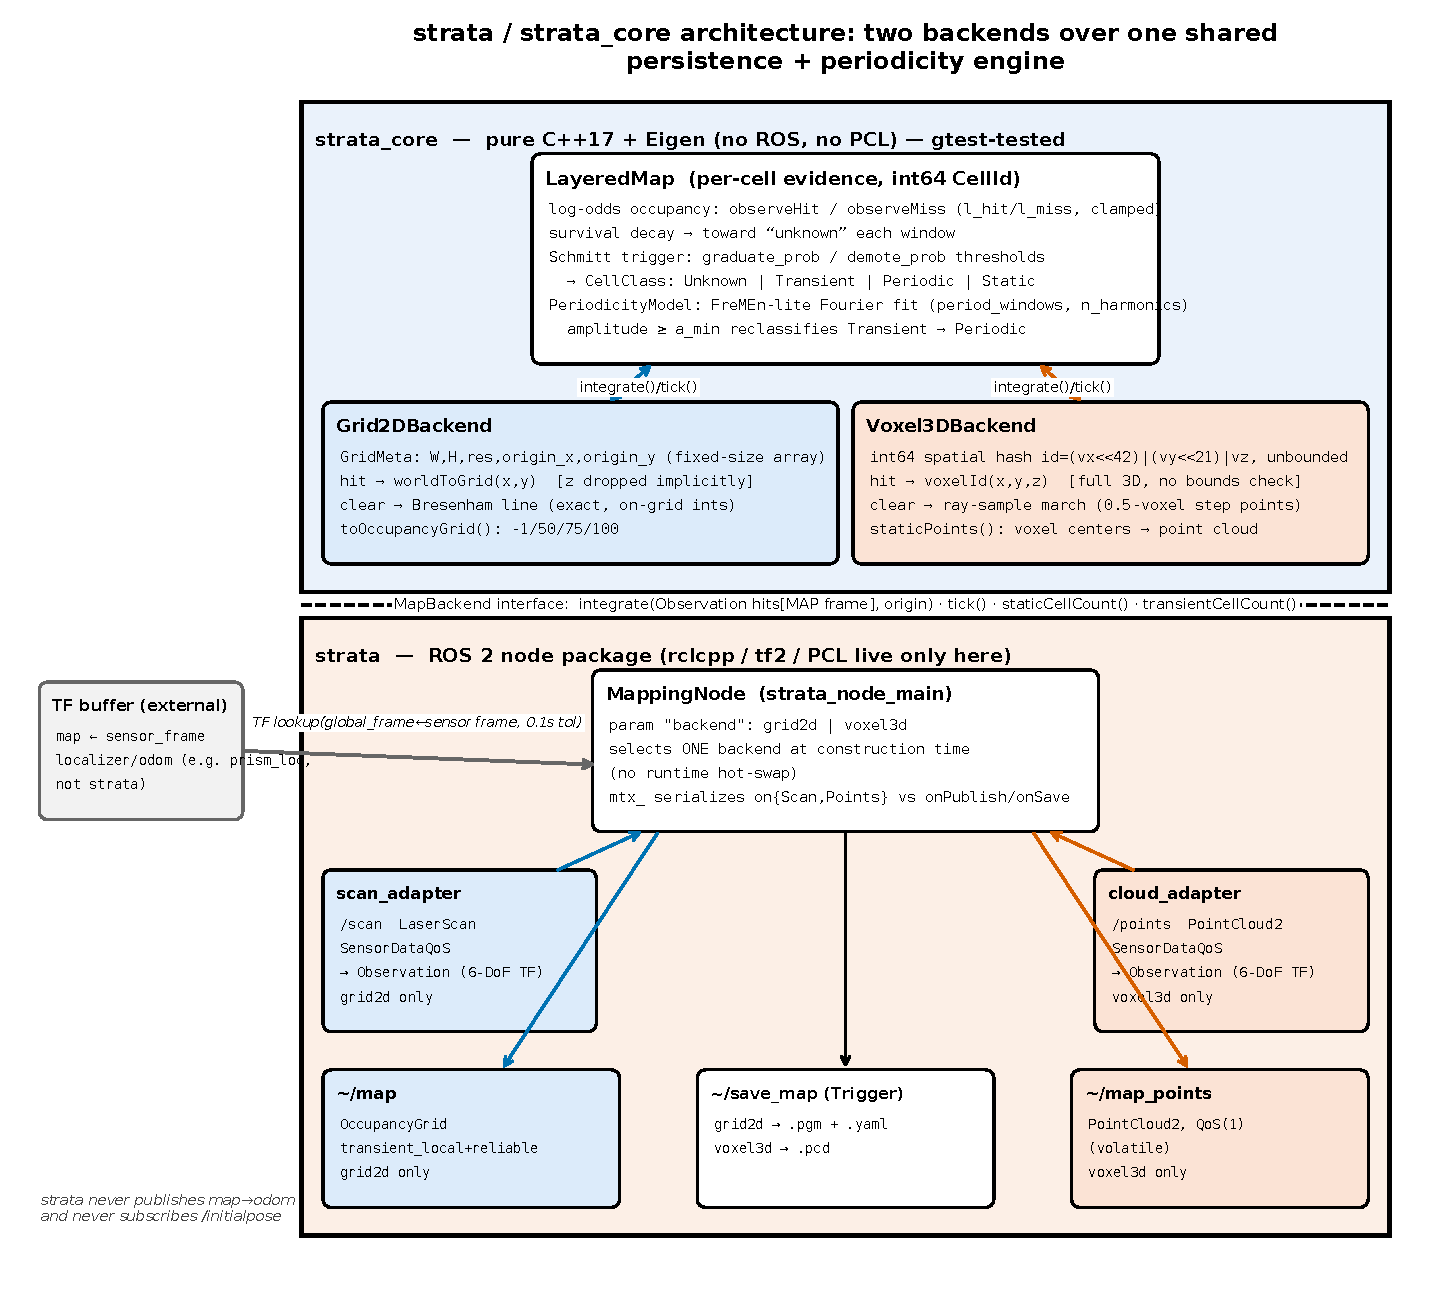
\includegraphics[width=\columnwidth]{figures/fig_architecture.pdf}
\caption{Two-band architecture of STRATA. The upper band is \texttt{strata\_core} (pure C++17
+ Eigen, no ROS or PCL, gtest-tested): one shared \texttt{LayeredMap}
persistence-and-periodicity engine, keyed by \texttt{int64} \texttt{CellId}, feeds two
sibling backend boxes \texttt{Grid2DBackend} and \texttt{Voxel3DBackend}. The lower band is
the \texttt{strata} ROS~2 node, where \texttt{MappingNode} selects one backend at
construction, its scan/cloud adapters convert messages to \texttt{Observation}s in the
map frame, and its timer publishes \texttt{\textasciitilde/map} / \texttt{\textasciitilde/map\_points} and services
\texttt{\textasciitilde/save\_map}. The two bands are split by the \texttt{MapBackend} interface line. The
external TF arrow (\texttt{map} $\to$ sensor frame) enters the node from outside the
diagram: STRATA consumes localization but never produces
it.}
\label{fig:architecture}
\end{figure}

\subsection{The \texttt{MapBackend} interface and the geometry-free invariant}
\label{sec:mapbackend}

\texttt{strata\_core::MapBackend} is a pure abstract base with four methods:

\begin{lstlisting}
struct Observation { std::vector<Eigen::Vector3d> hits; };  // endpoints, MAP frame
class MapBackend {
  virtual void integrate(const Observation& obs,
                         const Eigen::Vector3d& sensor_origin_map) = 0;
  virtual bool tick() = 0;
  virtual std::size_t staticCellCount() const = 0;
  virtual std::size_t transientCellCount() const = 0;
};
\end{lstlisting}

\texttt{Observation::hits} is a flat list of 3D endpoints already expressed in the map
frame; producing it from a sensor message and a \texttt{sensor\_to\_map} transform is
the caller's job, so the backend never touches TF. \texttt{integrate()} performs one
discrete map update from one sweep or cloud: for each hit it clears the
free-space cells between \texttt{sensor\_origin\_map} and the hit via a backend-specific
ray operation, then registers the hit itself as an occupied observation.
\texttt{tick()} advances the temporal window and returns whether a window boundary was
crossed. \texttt{staticCellCount()} and \texttt{transientCellCount()} are read-only
introspection forwarded to the shared classifier.

Both concrete backends hold a \texttt{LayeredMap} member and satisfy the interface
purely by translating world-frame geometry into \texttt{int64} \texttt{CellId} keys that
\texttt{LayeredMap} accumulates evidence for. This is the load-bearing design
invariant: \textbf{the only per-backend code is point$\to$id mapping and the
free-space ray walk; the occupancy/persistence/periodicity classifier is shared
by composition, not duplicated per dimension.} \texttt{LayeredMap} and
\texttt{PeriodicityModel} hold no coordinates, no resolution, and no origin --- only
integer ids --- so the identical engine drives both 2D and 3D. The consequence,
which the evaluation returns to, is that any cross-backend behavioral
divergence or cost gap must originate in the geometry layer, because that is
the only layer that differs.

\subsection{Backend selection}
\label{sec:selection}

Selection is a single string ROS parameter, \texttt{backend} (\texttt{"grid2d"} or
\texttt{"voxel3d"}), read once in the node constructor. It is not polymorphic dispatch
over a \texttt{MapBackend*}: the node holds both \texttt{std::unique\_ptr<Grid2DBackend>} and
\texttt{std::unique\_ptr<Voxel3DBackend>} as separate members, and an \texttt{if}/\texttt{else} at
construction instantiates exactly one of them, leaving the other null, and
wires up the backend-specific parameters, publisher, and subscriber. We use a
compile-time interface plus one runtime switch rather than \texttt{dlopen}-based
plugin loading. At two backends, \texttt{pluginlib} \cite{ros2pluginlib} would add a
registration and discovery mechanism whose cost is not repaid until the backend
count grows; we defer that machinery until it is. Both branches read every
\texttt{LayeredMapParams} field through a common helper, so the persistence and
periodicity tuning surface is backend-independent by construction.

\subsection{ROS~2 I/O contract}
\label{sec:io}

The node is \texttt{strata::MappingNode}, default node name \texttt{strata}. It looks up
\texttt{global\_frame} (default \texttt{map}) $\leftarrow$ sensor frame on every incoming
scan or cloud, at the message stamp, as a full 6-DoF \texttt{Eigen::Isometry3d}; there
is no yaw-only flattening on the input side. Lookup failures are caught and
rate-throttled rather than fatal, and that scan or cloud is dropped. STRATA is
mapping-only: it neither subscribes to \texttt{/initialpose} nor broadcasts
\texttt{map}$\to$\texttt{odom}. Pose must already be published on TF by an external
localizer. A single mutex serializes integration against publish and save.

\begin{table}[t]
\centering
\caption{ROS~2 input/output contract of the \texttt{strata} node.}
\label{tbl:io}
\footnotesize
\begin{tabular}{@{}p{0.09\columnwidth}p{0.30\columnwidth}p{0.28\columnwidth}p{0.20\columnwidth}@{}}
\toprule
Dir. & Name & Type / QoS & Condition \\
\midrule
Sub & \texttt{scan\_topic} (\texttt{/scan}) & \texttt{LaserScan}, SensorData & grid2d only \\
Sub & \texttt{points\_topic} (\texttt{/points}) & \texttt{PointCloud2}, SensorData & voxel3d only \\
Pub & \texttt{\textasciitilde/map} & \texttt{OccupancyGrid}, QoS(1) TL reliable & grid2d only \\
Pub & \texttt{\textasciitilde/map\_points} & \texttt{PointCloud2}, QoS(1) volatile & voxel3d only \\
Srv & \texttt{\textasciitilde/save\_map} & \texttt{Trigger}, default & both (.pgm+.yaml / .pcd) \\
Timer & \texttt{publish\_period} (1.0~s) & --- & drives publishing, both \\
\bottomrule
\end{tabular}
\end{table}

The occupancy-value convention on \texttt{\textasciitilde/map} and saved files is: unknown $-1$,
transient 50, periodic 75, static 100. For voxel3d, only the static-cell
set is emitted as points on \texttt{\textasciitilde/map\_points}.

\section{The Layered Map Engine}
\label{sec:method}

This section specifies the engine as implemented in \texttt{strata\_core}. All
equations are transcribed from the source, not from the design specification;
where the two disagree, \S\ref{sec:specdiff} documents the difference. Symbols follow
the notation used throughout the paper: $\ell$ is a cell's log-odds occupancy
evidence, $p=\sigma(\ell)$ its occupancy probability, $t$ the window (phase)
index, $H$ the harmonic count, $T$ the base period, and $\lambda$ the survival
decay.

\subsection{Per-frame accumulation and windowing}
\label{sec:windowing}

Each \texttt{observeHit(id)} / \texttt{observeMiss(id)} only increments the cell's window
counters, \texttt{window\_hits} or \texttt{window\_misses}; it performs no log-odds
arithmetic. Cells are created lazily on first touch, with $\ell=0$,
\texttt{observations=0}, and \texttt{graduated=false}. \texttt{tick()} advances the integration
counter and closes a window on the interval boundary:

\begin{equation}
\small
\begin{split}
\text{closeWindow} \iff\ & \big(\texttt{layer\_interval}\le 1\big)\ \lor\ \\
& \big(\texttt{integration\_count} \bmod \texttt{layer\_interval} = 0\big).
\end{split}
\end{equation}

The layered update, \texttt{endWindow()}, then runs once over \textbf{all} live cells. With
window counts $h_w$ and $m_w$, each cell's window is scored:

\begin{equation}
\begin{split}
\text{touched}&=[\,h_w>0 \lor m_w>0\,],\quad
\text{occ}=[\,h_w>0\,],\\
\text{free}&=[\,h_w=0 \land m_w>0\,].
\end{split}
\end{equation}

A single hit outweighs any number of misses in the same window.

\subsection{Log-odds persistence with survival decay}
\label{sec:logodds}

For \textbf{touched} cells only, the engine applies one log-odds increment
(an inverse-sensor-model update in the sense of \cite{thrun2005probabilistic}),
multiplies by the survival decay $\lambda$, and clamps:

\begin{equation}
\ell \leftarrow \operatorname{clamp}\!\Big(\lambda\big(\ell +
\underbrace{[\text{occ}]\,l_{\text{hit}} + [\text{free}]\,l_{\text{miss}}}_{\text{one increment}}\big),\;
l_{\min},\, l_{\max}\Big),
\end{equation}
\begin{equation}
\operatorname{clamp}(x,a,b)=\min\!\big(b,\max(a,x)\big),
\end{equation}

with occupancy probability $p=\sigma(\ell)=1/(1+e^{-\ell})$. The survival
multiplier is a constant-rate special case of the Persistence Filter forgetting
model \cite{rosen2016persistence}.

\textbf{Ordering note (load-bearing).} The decay multiplies the \emph{already-incremented}
value, so the fresh hit or miss is itself attenuated by $\lambda$ in the same
window. This is not the classic decay-then-add order. One consequence is the
decayed fixed point of repeated hits,
$\ell^\star=\lambda\,l_{\text{hit}}/(1-\lambda)\approx 27.5$, which the clamp
caps at $l_{\max}=5$, giving $p_{\max}=\sigma(5)\approx 0.9933$. With the
defaults, $p_{\text{grad}}=0.8$ corresponds to $\ell\ge\ln 4\approx 1.386$ and
$p_{\text{prune}}=0.05$ to $\ell<\ln(1/19)\approx -2.944$.

\subsection{Schmitt-trigger graduation and demotion}
\label{sec:schmitt}

After the log-odds update, $p$ and the periodicity amplitude $a$
(\S\ref{sec:periodicity}) are recomputed for \textbf{every} cell, touched or not, and the
\texttt{graduated} flag $g$ is updated by a two-sided Schmitt trigger:

\begin{equation}
\begin{split}
\textbf{graduate:}\quad & \lnot g \ \land\ \lnot\text{periodic}\ \land\
p \ge p_{\text{grad}}\ \land\ \\
& \text{observations}\ge N_{\min}\
\Rightarrow\ g\leftarrow\text{true},
\end{split}
\end{equation}

\begin{equation}
\textbf{demote:}\quad g \ \land\ \big(p \le p_{\text{dem}}\ \lor\
\text{periodic}\big)\ \Rightarrow\ g\leftarrow\text{false}.
\end{equation}

The interval $[p_{\text{dem}},\,p_{\text{grad}}]$ is the hysteresis band that
suppresses flicker at the static boundary; the motivation is the same
observation-consistency argument as in dynamic-object removal by
reverting \cite{kim2020removert}. Two periodicity guards go beyond a bare
threshold rule: \texttt{!periodic} blocks a strongly periodic cell from ever
graduating to Static, and \texttt{|| periodic} force-demotes a graduated cell that
later reveals periodicity. The two rules cannot fight in one window, because
graduation requires $\lnot\text{periodic}$ and
$p\ge p_{\text{grad}}>p_{\text{dem}}$.

\subsection{FreMEn-lite periodicity}
\label{sec:periodicity}

In parallel with occupancy, each touched cell (when \texttt{enable\_periodicity}) feeds
an incremental Fourier model in the spirit of FreMEn \cite{krajnik2017fremen}. With
the per-window occupancy sample $v=[\text{occ}]\in\{0,1\}$ and phase index $t$,
\texttt{gather} accumulates:

\begin{equation}
n \mathrel{+}= 1,\quad S_0 \mathrel{+}= v,
\end{equation}
\begin{equation}
\begin{split}
C_k &\mathrel{+}= v\cos\!\big((k{+}1)\omega t\big),\\
S_k &\mathrel{+}= v\sin\!\big((k{+}1)\omega t\big),\quad k=0..H{-}1,
\end{split}
\end{equation}
\begin{equation}
\omega = \frac{2\pi}{\max(1,\,T)}.
\end{equation}

Here $n$ counts \textbf{touched windows fed to gather}, not elapsed windows. The
phase prediction at window $t$ is

\begin{equation}
\begin{split}
\hat p(t)=\operatorname{clip}_{[0,1]}\Bigg(\frac{S_0}{n}+\sum_{k=0}^{H-1}
\Big[a_k\cos\!\big((k{+}1)\omega t\big)\ + \\
b_k\sin\!\big((k{+}1)\omega t\big)\Big]\Bigg),
\end{split}
\end{equation}

with DC term equal to the empirical mean $S_0/n$ and harmonic coefficients
$a_k=2C_k/n$, $b_k=2S_k/n$. The dominant-harmonic amplitude and the periodicity
test are

\begin{equation}
a=\begin{cases}0, & n < T\\[4pt]
\displaystyle\max_{0\le k<H}\sqrt{a_k^2+b_k^2}, & n \ge T\end{cases}
\end{equation}
\begin{equation}
\text{periodic}=\texttt{enable\_periodicity}\ \land\ a \ge a_{\min}.
\end{equation}

The $n\ge T$ gate means a sparsely observed cell needs $T$ touches before its
amplitude is trusted, which can span far more than $T$ elapsed windows.

\subsection{Cell-class state machine and pruning}
\label{sec:states}

At the end of each window, cells below confidence are erased:

\begin{equation}
\text{erase cell} \iff \lnot g\ \land\ p < p_{\text{prune}}\ \land\
a < a_{\min}.
\end{equation}

Static cells ($g$) and periodic cells ($a\ge a_{\min}$) are never pruned;
pruning a cell also erases its FreMEn coefficients. A snapshot classifier reads
out one of four states by a priority ladder:

\begin{equation}
\begin{split}
\text{absent}&\to\text{Unknown};\quad g\to\text{Static};\\
(\texttt{enable}\land a\ge a_{\min})&\to\text{Periodic};\quad
p\ge p_{\text{prune}}\to\text{Transient};\\
&\text{else}\to\text{Unknown}.
\end{split}
\end{equation}

The full transition table is Table~\ref{tbl:states}. Note that a present cell classifies
Unknown when $p<p_{\text{prune}}$ and it is neither periodic nor graduated --- the
same condition under which it is generally pruned in the same window.

\begin{table*}[t]
\centering
\caption{Cell-class transitions, all evidence-driven and evaluated at window close.}
\label{tbl:states}
\begin{tabular}{@{}lll@{}}
\toprule
From & To & Trigger \\
\midrule
(implicit) Unknown & Transient & first \texttt{observeHit/Miss}: cell created, $\ell{=}0\Rightarrow p{=}0.5\ge p_{\text{prune}}$ \\
Transient & Static & $p\ge p_{\text{grad}}\land\text{obs}\ge N_{\min}\land\lnot\text{periodic}$ (graduate) \\
Transient & Periodic & $a\ge a_{\min}$ (needs $n\ge T$ touched windows) \\
Transient & Unknown (erased) & $p<p_{\text{prune}}\land a<a_{\min}\land\lnot g$ (prune) \\
Static & Transient / Periodic / Unknown & demote ($p\le p_{\text{dem}}\lor\text{periodic}$), then re-classified by ladder \\
Periodic & Transient / Unknown & $a$ falls below $a_{\min}$ (then subject to prune) \\
Periodic & --- & never graduates (\texttt{!periodic} guard), never pruned while $a\ge a_{\min}$ \\
Static & --- & never pruned while $g$ \\
\bottomrule
\end{tabular}
\end{table*}

The complete per-window update is Algorithm~1.

\begin{lstlisting}
Algorithm 1  endWindow(): one layered update per closed window, over all live cells

  for each live cell c:                       # main update pass
      touched <- [h_w>0 or m_w>0]
      occ     <- [h_w>0]
      free    <- [h_w=0 and m_w>0]
      if touched:
          l  <- l + [occ]*l_hit + [free]*l_miss   # one log-odds increment
          l  <- lambda * l                        # decay attenuates the fresh increment
          l  <- clamp(l, l_min, l_max)
          observations <- observations + 1
          if enable_periodicity:
              gather(c, occ, t)                   # n+=1; S0+=v; Ck+=v cos((k+1)w t); Sk+=v sin((k+1)w t)
      p <- sigma(l);  a <- amplitude(c)           # recomputed for ALL cells, touched or not
      periodic <- enable_periodicity and a >= a_min
      if not g and not periodic and p >= p_grad and observations >= N_min:
          g <- true                               # graduate -> Static
      else if g and (p <= p_dem or periodic):
          g <- false                              # demote
      reset h_w <- 0, m_w <- 0
  for each live cell c:                       # prune pass
      if not g and p < p_prune and a < a_min:
          erase c and its FreMEn coefficients
  t <- t + 1
\end{lstlisting}

The window update is $O(N\cdot H)$ for $N$ live cells and $H$ constant, hence
$O(N)$; it iterates all cells, including untouched ones, because the Schmitt
and prune decisions read the recomputed $p$ and $a$ of every cell. Between
window closes a frame is $O(1)$ per endpoint plus the backend ray cost.

\subsection{Geometry backends}
\label{sec:backends}

The two backends differ only in how a world point becomes a \texttt{CellId} and how the
free-space ray is walked; both delegate all evidence updates to the shared
\texttt{LayeredMap}.

\texttt{Grid2DBackend} addresses a fixed-size, fixed-origin 2D array described by
\texttt{GridMeta} $=\{$\texttt{width, height, resolution, origin\_x, origin\_y}$\}$. It buckets
each hit's $(x,y)$ (dropping $z$) into a row-major id
$\texttt{gridCellId}(m,g_x,g_y)=g_y\cdot\texttt{width}+g_x$; points outside the
array are dropped. Free space is cleared with integer Bresenham's line algorithm
from the sensor cell to the hit cell, calling \texttt{observeMiss} on every
intermediate cell strictly between the endpoints, so the hit cell receives only
\texttt{observeHit}. Rendering to \texttt{nav\_msgs/OccupancyGrid} initializes every cell to
$-1$, then overwrites in ascending confidence order transient$\to$50,
periodic$\to$75, static$\to$100, so static wins any tie.

\texttt{Voxel3DBackend} has no fixed extent; the map grows through the hash map. Each
axis is floor-divided by \texttt{voxel\_size} and offset by $\texttt{kOff}=1\ll 20$ to
keep the per-axis index non-negative, and the three 21-bit
($\texttt{kBits}=21$) fields are packed into one 64-bit key,
$\text{id}=(v_x\ll 42)\,|\,(v_y\ll 21)\,|\,v_z$; \texttt{voxelCenter} is the exact
inverse, returning $(v+0.5)\cdot\texttt{voxel\_size}$ per axis. This gives O(1)
hashing and a per-axis range far larger than any practical map. Free space is
cleared by ray-sample marching, not geometric voxel traversal: the ray is
subdivided into $\lceil\text{len}/(0.5\cdot\texttt{voxel\_size})\rceil$
half-voxel steps, and each interior sample is hashed to its containing voxel and
marked \texttt{observeMiss}. This is simpler than exact traversal but can over-sample a
long ray and can skip a thin voxel when the step count rounds down. The hit is
always \texttt{observeHit}, with no bounds check because the hash grows to fit.
\texttt{staticPoints()} maps the static-cell set through \texttt{voxelCenter} to a point
cloud. Table~\ref{tbl:backends} contrasts the two.

\begin{table*}[t]
\centering
\caption{The two geometry backends. All persistence and periodicity logic is shared; only these two rows of behavior differ.}
\label{tbl:backends}
\begin{tabular}{@{}lll@{}}
\toprule
 & \texttt{Grid2DBackend} & \texttt{Voxel3DBackend} \\
\midrule
Cell addressing & 2D array index via \texttt{GridMeta} (fixed $W\times H$, fixed origin) & 3D spatial hash, unbounded, \texttt{int64} packed key \\
Hit dimensionality & $x,y$ (z dropped by projection) & $x,y,z$ (full volumetric) \\
Free-space ray & Bresenham line (exact, on-grid) & ray-sample march at 0.5-voxel step (approximate, off-grid) \\
Growth & none --- pre-sized at construction & unbounded --- hash grows with exploration \\
Output & \texttt{nav\_msgs/OccupancyGrid} (dense $-1$/50/75/100) & static voxel centers $\to$ \texttt{PointCloud2} \\
\bottomrule
\end{tabular}
\end{table*}

\subsection{Parameters}
\label{sec:params}

Table~\ref{tbl:params} lists the engine's tunable parameters with their defaults, which
are identical between the struct definition and both shipped YAML files. Geometry
and node parameters (\texttt{grid\_width} 400, \texttt{grid\_height} 400, \texttt{grid\_resolution}
0.05~m, \texttt{grid\_origin\_\{x,y\}} $-10.0$~m for grid2d; \texttt{voxel\_size} 0.2~m for voxel3d;
frame names, topics, \texttt{publish\_period} 1.0~s) are not part of the engine math.

\begin{table}[t]
\centering
\caption{Engine parameters and defaults (struct and \texttt{params/*.yaml} agree).}
\label{tbl:params}
\begin{tabular}{@{}p{0.30\columnwidth}p{0.10\columnwidth}p{0.50\columnwidth}@{}}
\toprule
Name & Default & Meaning \\
\midrule
\texttt{layer\_interval} & 10 & integration ticks per layered-update window \\
\texttt{l\_hit} & 0.85 & log-odds increment on an occupied window \\
\texttt{l\_miss} & $-0.4$ & log-odds increment on a free window \\
\texttt{l\_min} & $-5.0$ & clamp lower bound (log-odds) \\
\texttt{l\_max} & 5.0 & clamp upper bound (log-odds) \\
\texttt{survival\_decay} ($\lambda$) & 0.97 & Persistence-Filter forgetting multiplier, per window \\
\texttt{graduate\_prob} ($p_{\text{grad}}$) & 0.8 & $p$ to promote $\to$ Static \\
\texttt{demote\_prob} ($p_{\text{dem}}$) & 0.45 & $p$ at/below which Static demotes (hysteresis floor) \\
\texttt{min\_observations} ($N_{\min}$) & 3 & min touched windows before a cell may graduate \\
\texttt{prune\_prob} ($p_{\text{prune}}$) & 0.05 & erase non-static, non-periodic cell below this $p$ \\
\texttt{enable\_periodicity} & true & run the FreMEn model \\
\texttt{periodic\_amplitude\_min} ($a_{\min}$) & 0.3 & dominant-harmonic magnitude to classify Periodic \\
\texttt{period\_windows} ($T$) & 24 & FreMEn base period; also amplitude-validity gate ($n\ge T$) \\
\texttt{n\_harmonics} ($H$) & 2 & Fourier harmonics tracked per cell \\
\bottomrule
\end{tabular}
\end{table}

Per-cell state is compact: \texttt{CellEvidence} is 24 bytes, plus roughly 32 bytes of
\texttt{unordered\_map} node overhead, giving the $\sim$56~B/cell footprint reported in the
evaluation when periodicity storage is excluded. A FreMEn-tracked cell adds a
\texttt{Coeff} record ($\sim$96~B payload at $H=2$), allocated only for cells touched at
least once with periodicity enabled.

\subsection{Implementation versus specification}
\label{sec:specdiff}

We document the code that ships, not the design prose. Three points where the
implementation diverges from \texttt{SPEC.md} are surfaced here rather than smoothed
over, because each changes the operational semantics.

\textbf{SPEC-DIFF \#1 (forgetting is coupled to re-observation).} The specification
states that decay happens "every window" and that "a cell that stops being
observed decays out." In code, the entire log-odds-and-clamp block of
\S\ref{sec:logodds} is inside \texttt{if (touched)}. An untouched cell --- out of the sensor
field of view, with neither a hit nor a miss that window --- does not decay; its
$\ell$ freezes. Forgetting therefore requires being re-observed as free (a miss
is a touch), so clutter fades only while it stays in the field of view, and
anything that leaves the field of view persists indefinitely. This is the most
consequential difference and is restated as an operational limitation in the
discussion.

\textbf{SPEC-DIFF \#2 (periodicity guards absent from the formal block).} The
specification's \S3.4 pseudocode omits the periodicity guards entirely, listing
graduate as \texttt{!graduated \&\& p >= graduate\_prob \&\& observations >= min\_observations}
and demote as \texttt{graduated \&\& p <= demote\_prob}. The \texttt{!periodic} and \texttt{|| periodic}
terms actually in the code (\S\ref{sec:schmitt}) appear only in prose and comments. A
method transcribed verbatim from that block would be wrong; the equations above
follow the code.

\textbf{SPEC-DIFF \#3 (amplitude gate counts touched windows, not elapsed time).} The
specification says amplitude is zero before \texttt{period\_windows} windows have
\emph{elapsed}. The code gates on $n<T$, where $n$ is the count of touched windows
(calls to \texttt{gather}), not elapsed wall or window time. A sparsely observed cell
needs $T$ touches, which can span far more than $T$ windows --- the mechanism
behind the low-duty periodicity miss reported in the evaluation.

\section{Evaluation (synthetic)}
\label{sec:eval}

\subsection{Setup}

All four experiments (E1--E4) are driven by a standalone harness in
\texttt{paper/experiments/} that links directly against the \texttt{strata\_core} sources ---
no ROS~2, no ament, no colcon. Reproduction from the repository root is a
single call, \texttt{bash paper/experiments/run\_all.sh}, which configures and builds
\texttt{strata\_core} and the four harness executables, runs each one, and writes the
CSVs in \texttt{paper/experiments/results/} from which every number and figure in
this section is taken; \texttt{strata\_core}'s own \texttt{ctest} suite (1/1) is checked
first, so the harness is only trusted once the unit-level behavior it builds
on is confirmed. Every stochastic experiment (E1--E3) seeds a single
\texttt{std::mt19937} from the fixed constant \texttt{kSeed = 12345}, recorded in each
CSV's \texttt{\#seed} row, so the reported precision/recall/F1/flicker/TPR/FPR
numbers are exactly reproducible. E4 additionally reads the wall clock to
time \texttt{integrate()}/\texttt{endWindow()} calls; its absolute microsecond figures are
therefore machine-dependent, while the live-cell counts it also reports are
deterministic (they follow only from ray geometry, not timing).

The four experiments map onto the two thesis claims of \S\ref{sec:system}--\ref{sec:method} (C2, C5)
differently. E1 and E4 probe \emph{backend-behavior equivalence}: both feed
identical hit/miss streams through \texttt{Grid2DBackend} and \texttt{Voxel3DBackend} and
compare the outcome, so any divergence is attributable only to the
geometry layer (point$\to$\texttt{CellId} mapping and the free-space ray walk),
since the classifier code both backends call is the same \texttt{LayeredMap}
instance type. E2 and E3, by contrast, drive \texttt{LayeredMap}/\texttt{PeriodicityModel}
directly, with no backend in the loop at all --- a choice that is itself an
argument for C1: because persistence, hysteresis, and periodicity are
implemented once, independent of \texttt{CellId} provenance, characterizing them
against \texttt{LayeredMap} directly is valid for whichever backend supplies the
cell ids in production. Each harness constructs its own \texttt{LayeredMapParams}
in code rather than loading the shipped YAML, so several values deviate from
the Table~\ref{tbl:params} production defaults; Table~\ref{tbl:eparams} lists every deviation,
per experiment, so the runs are reproducible without reading the harness
source. Three deviations are common to interpreting the results below: all
four harnesses run at \texttt{layer\_interval} 1 (one window per integration tick,
against the production default of 10), so "window" and "frame" coincide in
every reported count; E1, E3, and E4 disable periodicity to isolate the
persistence layer (E2 is the only run that exercises the FreMEn model); and
E4 and E2 both set \texttt{survival\_decay} 1.0 (no forgetting). E2 in particular
raises all six of the log-odds/graduation defaults it touches
($l_{\text{hit}}$ 1.0, $l_{\text{miss}}$ $-1.0$, $\lambda$ 1.0,
$p_{\text{grad}}$ 0.9, $p_{\text{dem}}$ 0.4, $N_{\min}$ 5) to drive its
detected-versus-pruned classification, and E3 lowers \texttt{prune\_prob} to 0.01 to
keep noisy walls alive; these are the values actually compiled into each
harness.

\begin{table}[t]
\centering
\caption{Per-experiment deviations from the Table~\ref{tbl:params} production defaults. ``---'' = default unchanged; ``swept'' = varied across the E3 configuration grid ($\lambda\in\{0.90,0.97,1.0\}$, \texttt{graduate\_prob} $\in\{0.6,0.7,0.8,0.9\}$, \texttt{demote\_prob} $\in\{0.3,0.5,\text{graduate\_prob}\}$); ``n/a'' = inert because periodicity is disabled in that run.}
\label{tbl:eparams}
\small
\begin{tabular}{@{}lllll@{}}
\toprule
Parameter (default) & E1 & E2 & E3 & E4 \\
\midrule
\texttt{layer\_interval} (10) & 1 & 1 & 1 & 1 \\
\texttt{enable\_periodicity} (true) & false & true & false & false \\
$l_{\text{hit}}$ (0.85) & --- & 1.0 & --- & --- \\
$l_{\text{miss}}$ ($-0.4$) & --- & $-1.0$ & --- & --- \\
\texttt{survival\_decay} (0.97) & --- & 1.0 & swept & 1.0 \\
\texttt{graduate\_prob} (0.8) & --- & 0.9 & swept & --- \\
\texttt{demote\_prob} (0.45) & --- & 0.4 & swept & --- \\
\texttt{min\_observations} (3) & --- & 5 & --- & --- \\
\texttt{prune\_prob} (0.05) & --- & --- & 0.01 & --- \\
\texttt{period\_windows} (24) & n/a & 8 & n/a & n/a \\
\texttt{n\_harmonics} (2) & n/a & 3 & n/a & n/a \\
\bottomrule
\end{tabular}
\end{table}

\subsection{E1 --- Static-layer map quality vs.\ time}

\textbf{Setup.} A ground-truth static cross of 161 cells (segment $y{=}60,
x\in[20,100]$ and $x{=}60, y\in[20,100]$) is hit every window, alongside
transient movers at three densities --- low/med/high = 5/25/100 fresh random
cells per window --- over 40 windows, run against both a $120\times120$
(resolution 1.0) \texttt{Grid2DBackend} and a 1.0-voxel \texttt{Voxel3DBackend}, with
periodicity disabled to isolate the persistence layer. Static-set
precision/recall/F1 against the 161-cell wall set is logged per window
(\texttt{results/e1\_static\_quality.csv}).

\begin{table}[t]
\centering
\caption{E1 --- final static-set precision/recall/F1, both backends, all three clutter densities.}
\label{tbl:e1}
\footnotesize
\begin{tabular}{@{}llccc@{}}
\toprule
backend & density & recall $=1$ & prec.\ @$39$ & F1 @$39$ \\
\midrule
grid2d & low (5/w) & window 3 & 1.0000 & 1.0000 \\
grid2d & med (25/w) & window 3 & 0.9938 & 0.9969 \\
grid2d & high (100/w) & window 3 & 0.9253 & 0.9612 \\
voxel3d & low (5/w) & window 3 & 1.0000 & 1.0000 \\
voxel3d & med (25/w) & window 3 & 0.9938 & 0.9969 \\
voxel3d & high (100/w) & window 3 & 0.9758 & 0.9877 \\
\bottomrule
\end{tabular}
\end{table}

\begin{figure}[t]
\centering
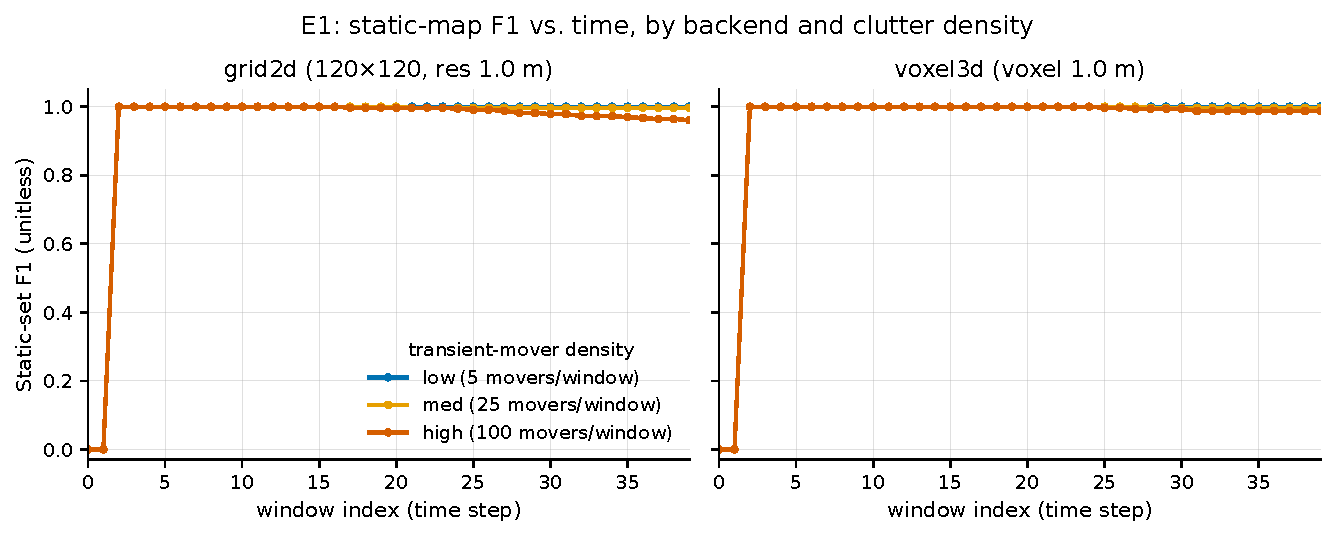
\includegraphics[width=\columnwidth]{figures/fig_e1_f1_vs_time.pdf}
\caption{E1: static-set F1 vs.\ window index, one panel per backend, one line per
clutter density. Both backends recover F1$\approx$1.0 within three windows;
the 100-movers/window regime is the only one with a visible
precision/F1 dip, and the dip is larger for
grid2d.}
\label{fig:e1}
\end{figure}

With $N_{\min}=3$, a cell needs three touched windows before it is eligible
to graduate; the CSV confirms recall jumps from 0 to 1.0 exactly at the
third window (window index $t{=}2$) for every one of the six
backend$\times$density combinations, and holds at 1.0 through $w{=}39$ in
every case --- no wall cell is ever demoted by clutter. The only errors are a
handful of false-positive statics that appear when a random mover happens to
re-hit the same cell often enough to graduate on its own; at low density
(5 movers/window) this never happens at all, and precision stays exactly
1.0 through $w{=}39$ for both backends. At medium density it saturates at a
single spurious cell (precision floors at 0.9938 and never falls further),
but at high density (100 movers/window) false statics keep accumulating
window over window --- from 162 predicted cells at $w{=}17$ (grid2d) /
$w{=}25$ (voxel3d) to 174 (grid2d) / 165 (voxel3d) by $w{=}39$ --- giving the
only material gap between backends:
precision 0.9253 (grid2d) vs.\ 0.9758 (voxel3d) at the final window. Both
backends run the identical \texttt{LayeredMap} graduation rule on the identical
mover stream; the gap traces to geometry, not the classifier --- \texttt{Grid2DBackend}
projects every hit onto a shared 2D $(x,y)$ cell (dropping $z$), so
independent movers collide into the same cell more often than in
\texttt{Voxel3DBackend}'s full 3D hash, and each collision is exactly the
accumulation event that produces a spurious static.

\subsection{E2 --- Periodicity detection}

\textbf{Setup.} Three periodic doors (\texttt{p8} 4-on/4-off, \texttt{p8} 2-on/6-off, \texttt{p4}
2-on/2-off, all detectable against the FreMEn base period $T{=}8$ with
$H{=}3$ harmonics), a constant wall, and four deterministic Bernoulli(0.5)
aperiodic movers as negative controls, are driven through the real
\texttt{LayeredMap} pipeline for 64 windows. Reported: per-cell final class against
ground truth (Periodic TPR/FPR), and FreMEn dominant-harmonic amplitude vs.\
observation length (\texttt{results/e2\_classification.csv},
\texttt{results/e2\_amplitude\_vs\_length.csv}, \texttt{results/e2\_summary.csv}).

\begin{table}[t]
\centering
\caption{E2 --- per-cell classification against ground truth ($a_{\min}=0.3$); Periodic TPR $=2/3$, FPR $=1/5$.}
\label{tbl:e2}
\small
\begin{tabular}{@{}p{0.30\columnwidth}p{0.13\columnwidth}p{0.13\columnwidth}p{0.10\columnwidth}p{0.13\columnwidth}@{}}
\toprule
cell & ground truth & final class & ampl.\ & note \\
\midrule
\texttt{door\_p8\_4on4off} (50\% duty) & periodic & Periodic & 0.653 & correct \\
\texttt{door\_p4\_2on2off} (50\% duty) & periodic & Periodic & 0.707 & correct \\
\texttt{door\_p8\_2on6off} (25\% duty) & periodic & Transient & --- & \textbf{miss} \\
\texttt{wall\_constant} & non-periodic & Static & $\approx$0 & correct \\
\texttt{aperiodic\_1} & non-periodic & Periodic & 0.329 & \textbf{FP} \\
\texttt{aperiodic\_0,\_2,\_3} & non-periodic & Transient & 0.14--0.25 & correct \\
\bottomrule
\end{tabular}
\end{table}

\begin{figure}[t]
\centering
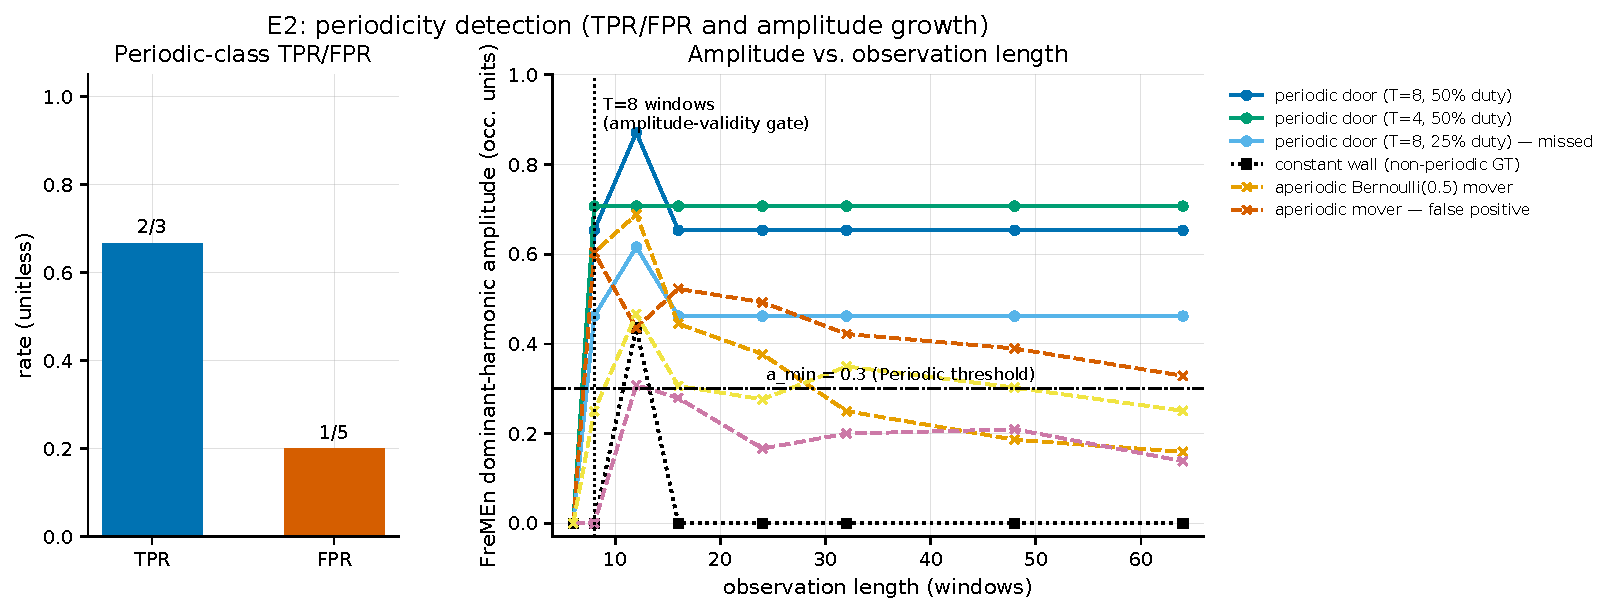
\includegraphics[width=\columnwidth]{figures/fig_e2_periodicity.pdf}
\caption{E2: (left) Periodic-class TPR/FPR bars; (right) FreMEn dominant-harmonic
amplitude vs.\ observation length for all 8 probe cells, with the
$a_{\min}=0.3$ threshold and the $n\ge T$ validity gate marked --- the two
50\%-duty doors clear the threshold cleanly, the 25\%-duty door is pruned
before it matures, and one aperiodic mover produces the false
positive.}
\label{fig:e2}
\end{figure}

Both 50\%-duty doors are detected cleanly: amplitude 0.653 and 0.707 clear
$a_{\min}=0.3$ by a wide margin. The one miss, the 25\%-duty door
(\texttt{door\_p8\_2on6off}), is a \textbf{prune/maturity race}, not a modeling failure:
the notes accompanying this harness report that the real pipeline prunes
this cell in roughly 10 of its 64 windows --- each 6-window vacant stretch
lets its log-odds fall below $p_{\text{prune}}$ while its FreMEn amplitude
is still 0 (the $n\ge T$ gate has not yet been reached), erasing its
accumulator state before periodicity can mature. The CSV's \texttt{ref\_amplitude}
column --- a non-pruning reference \texttt{PeriodicityModel} fed the identical
occupancy stream --- reads 0.46194 for this same cell, comfortably above
$a_{\min}$, confirming the signal itself is periodic and detectable; the
miss is specifically an interaction between pruning and the touched-window
amplitude gate. The lone false positive, \texttt{aperiodic\_1} at amplitude 0.329,
is a Bernoulli(0.5) cell whose Fourier energy over 64 windows happens to
clear the 0.30 threshold by a small margin (0.029 above $a_{\min}$) --- the
kind of chance alignment expected from a fixed-length random negative
control rather than a systematic classifier flaw. The amplitude-vs-length
data also confirms the validity gate operates as specified: for
\texttt{door\_p8\_4on4off}, amplitude is exactly 0 at observation length 6 ($n<T{=}8$)
and jumps to 0.653 at length 8 ($n\ge T$), where it then stabilizes.

\subsection{E3 --- Sensitivity: hysteresis band and decay}

\textbf{Setup.} 50 ground-truth wall cells are observed occupied with probability
0.6 each window (noisy) alongside 10 fresh movers/window, over 80 windows,
with the identical noise sequence replayed for every configuration in the
sweep. The sweep spans \texttt{graduate\_prob} $\in\{0.6,0.7,0.8,0.9\}$
$\times$ \texttt{demote\_prob} (a low floor 0.3, a mid floor 0.5, and the degenerate
\texttt{demote\_prob == graduate\_prob}, i.e.\ zero hysteresis band)
$\times$ \texttt{survival\_decay} $\in\{0.90,0.97,1.0\}$ --- 36 configurations total.
Reported: final Static-layer F1 and the count of per-window \texttt{isStatic}
flicker transitions (\texttt{results/e3\_sensitivity.csv}).

\begin{table}[t]
\centering
\caption{E3 --- selected sweep configurations (full 36-row sweep in the CSV); identical replayed noise throughout.}
\label{tbl:e3}
\small
\begin{tabular}{@{}p{0.10\columnwidth}p{0.13\columnwidth}p{0.10\columnwidth}p{0.10\columnwidth}p{0.10\columnwidth}p{0.10\columnwidth}@{}}
\toprule
grad. & dem. & band & decay & flicker & F1 \\
\midrule
0.9 & 0.9 (deg.) & 0 & 0.90 & \textbf{574} & \textbf{0.810} \\
0.8 & 0.8 (deg.) & 0 & 0.90 & 343 & 0.947 \\
0.7 & 0.7 (deg.) & 0 & 0.90 & 250 & 0.980 \\
0.9 & 0.9 (deg.) & 0 & 0.97 & 150 & 1.000 \\
0.9 & 0.9 (deg.) & 0 & 1.00 & 122 & 1.000 \\
0.9 & 0.3 & 0.6 & 0.90 & 54 & 1.000 \\
0.9 & 0.3 & 0.6 & 0.97 & 52 & 1.000 \\
0.9 & 0.3 & 0.6 & 1.00 & \textbf{52} & \textbf{1.000} \\
\bottomrule
\end{tabular}
\end{table}

\begin{figure}[t]
\centering
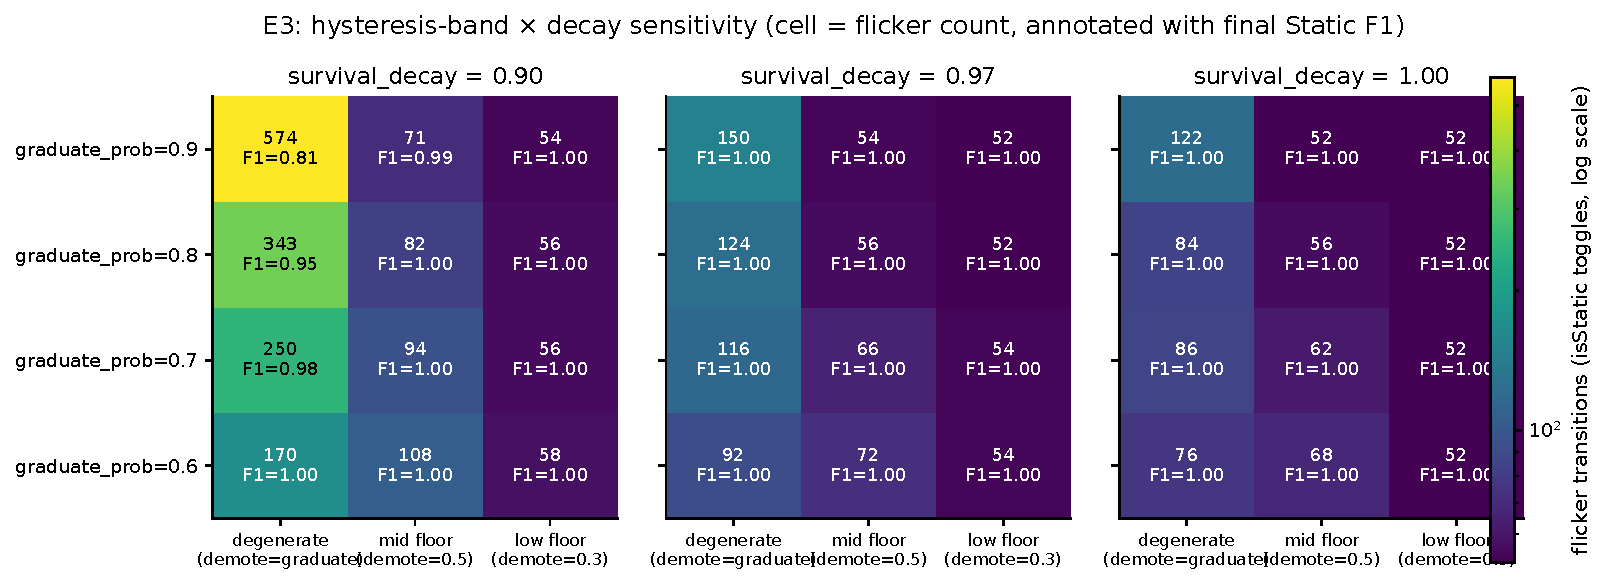
\includegraphics[width=\columnwidth]{figures/fig_e3_sensitivity.pdf}
\caption{E3: three heatmap panels (one per \texttt{survival\_decay}); rows =
\texttt{graduate\_prob}, columns = hysteresis-band width, cells colored by
flicker-transition count (log scale) and annotated with the raw count and
final F1 --- the degenerate (zero-band) column drives both the worst flicker
and the worst F1 at every decay
setting.}
\label{fig:e3}
\end{figure}

Removing hysteresis is the single largest effect in the sweep: at
\texttt{graduate\_prob = demote\_prob = 0.9}, \texttt{survival\_decay = 0.90} (the worst
degenerate configuration), the wall layer flickers 574 times and loses
19\% of its final F1 (0.810, recall collapses to 0.68), while a
same-noise, same-decay run with the hysteresis band widened to 0.6
(\texttt{demote\_prob = 0.3}) flickers only 54 times at F1 1.000 --- the band alone
accounts for a $>10\times$ reduction in flicker. The degenerate
(zero-band) configurations are also internally monotonic in threshold: at
\texttt{survival\_decay = 0.90}, flicker rises with the coincident threshold value
(250 at 0.7, 343 at 0.8, 574 at 0.9) even though a higher threshold is
ordinarily the more conservative, more "static" setting --- a threshold pair
with no gap between graduate and demote is not a substitute for a
hysteresis band, regardless of where that pair sits.
\texttt{survival\_decay} is the second-order effect: holding the worst degenerate
threshold pair (0.9/0.9) fixed, flicker falls monotonically as forgetting
slows --- 574 at $\lambda{=}0.90$, 150 at $\lambda{=}0.97$, 122 at
$\lambda{=}1.0$ --- because faster decay lets noisy log-odds cross the
(here, coincident) threshold more often. With a wide hysteresis band,
\texttt{survival\_decay} barely matters (52--54 flicker across all three decay
settings at the best band): hysteresis, not decay, is what keeps the
static layer stable.

\subsection{E4 --- Throughput and memory}

\textbf{Setup.} 150 random hits per window over 20 windows, for \texttt{Grid2DBackend}
vs.\ \texttt{Voxel3DBackend} at three nominal extents (100/250/500, resolution/voxel
size 1.0), periodicity disabled. Reported: mean per-\texttt{integrate()} call
latency, mean per-\texttt{endWindow()} cell-update rate, final live-cell count, and
estimated memory at the fixed 56~B/cell footprint documented in \S\ref{sec:method}
(\texttt{CellEvidence} 24~B + $\approx$32~B \texttt{unordered\_map} node overhead, with
FreMEn storage excluded since periodicity is off in this run)
(\texttt{results/e4\_throughput.csv}).

\begin{table}[t]
\centering
\caption{E4 --- per-call latency, throughput, live-cell count, and estimated memory, both backends, all three extents. Absolute $\mu$s are single-machine wall-clock samples; live-cell counts (and the ratios derived from them) are geometry-determined and reproducible.}
\label{tbl:e4}
\small
\begin{tabular}{@{}llrrrr@{}}
\toprule
backend & extent & $\mu$s/\texttt{intg.} & updates/s & live cells & memory \\
\midrule
grid2d & $100^2$ & 320.8 & $9.41{\times}10^{6}$ & 8{,}553 & 479~KB \\
voxel3d & $100^2$ & 4{,}796.8 & $7.06{\times}10^{6}$ & 85{,}399 & 4.78~MB \\
grid2d & $250^2$ & 1{,}702.6 & $1.07{\times}10^{7}$ & 45{,}657 & 2.56~MB \\
voxel3d & $250^2$ & 18{,}469.5 & $4.46{\times}10^{6}$ & 295{,}300 & 16.5~MB \\
grid2d & $500^2$ & 6{,}548.9 & $8.64{\times}10^{6}$ & 150{,}096 & 8.41~MB \\
voxel3d & $500^2$ & 35{,}958.3 & $4.45{\times}10^{6}$ & 661{,}410 & 37.0~MB \\
\bottomrule
\end{tabular}
\end{table}

\begin{figure}[t]
\centering
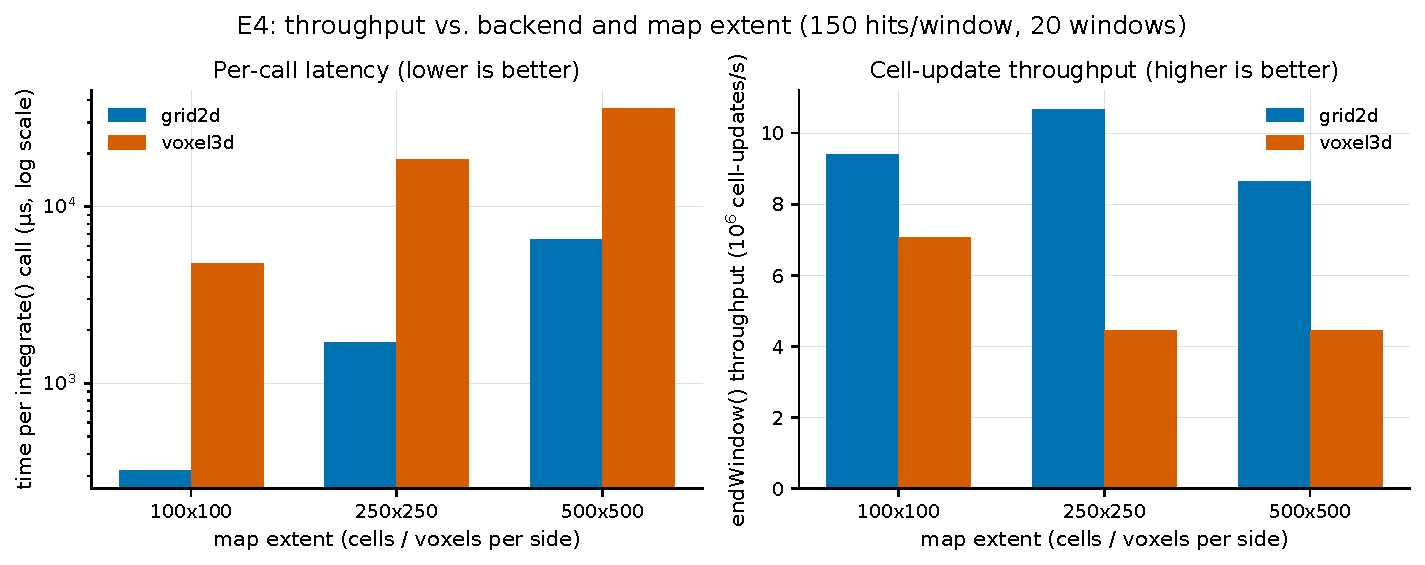
\includegraphics[width=\columnwidth]{figures/fig_e4_throughput.pdf}
\caption{E4: grouped bars by backend $\times$ extent --- per-\texttt{integrate()}
latency in $\mu$s (log scale, left) and \texttt{endWindow()} cell-update throughput in
$10^6$ updates/s (right). grid2d is cheaper per call than voxel3d at every
tested extent; the gap tracks voxel3d's larger live-cell
count.}
\label{fig:e4}
\end{figure}

At every tested extent, \texttt{Grid2DBackend}'s \texttt{integrate()} call is cheaper than
\texttt{Voxel3DBackend}'s at the identical nominal extent and hit rate --- by
$4{,}796.8/320.8\approx14.9\times$ at $100^2$, $18{,}469.5/1{,}702.6\approx
10.8\times$ at $250^2$, and $35{,}958.3/6{,}548.9\approx5.5\times$ at
$500^2$, the multiple shrinking as extent grows. The live-cell counts
explain why: \texttt{Voxel3DBackend} ends each run holding
$85{,}399/8{,}553\approx10.0\times$, $295{,}300/45{,}657\approx6.5\times$,
and $661{,}410/150{,}096\approx4.4\times$ as many cells as \texttt{Grid2DBackend}
at the same extent, because its free-space ray-sample march (\S\ref{sec:backends}) walks a
full 3D volume and spawns far more traversed voxels than \texttt{Grid2DBackend}'s
exact 2D Bresenham clear over the same nominal footprint --- the same
geometric asymmetry that drives the latency gap also drives the cell-count
gap, and both narrow together as the extent grows and the ray paths (and
hence the per-ray voxel counts) become a smaller fraction of the total
volume. Memory is exactly what a flat 56~B/cell predicts: estimated memory
tracks live-cell count linearly across every row of Table~\ref{tbl:e4} with no
additional constant, topping out at 37.0~MB for the largest 3D
configuration tested (661,410 cells $\times$ 56~B) --- inexpensive even at
the largest map in this sweep. Absolute microsecond values here are
single-run wall-clock measurements on one machine and are not claimed to be
portable; the live-cell counts, and the ratios and memory figures derived
from them, follow only from ray/hash geometry and reproduce under the fixed
seed regardless of machine.

\subsection{Synthesis}

Across E1--E4, the two backends behave as one engine wearing two geometries,
exactly as C1 asserts by construction: E1's near-identical F1 trajectories
(both backends graduate the wall by the third window and hold recall 1.0
through $w{=}39$) and E4's flat 56~B/cell tracking live-cell count are the
empirical face of "no per-dimension logic or cost," since \texttt{LayeredMap} and
\texttt{PeriodicityModel} --- exercised directly and identically in E2 and E3 --- never
see which backend produced the \texttt{CellId} they are updating. The two places
where the backends \emph{do} diverge are both traced, not merely asserted, to
geometry rather than to the shared classifier: E1's high-clutter precision
gap (0.9253 vs.\ 0.9758) follows from \texttt{Grid2DBackend}'s 2D $z$-projection
colliding independent movers into shared cells more often than
\texttt{Voxel3DBackend}'s full-3D hash, and E4's per-call latency gap
(5.5--14.9$\times$, narrowing with extent) follows from \texttt{Voxel3DBackend}'s
free-space ray-sample march spawning 4.4--10.0$\times$ more live voxels than
\texttt{Grid2DBackend}'s exact line clear at the same nominal extent. E2 and E3,
run once against \texttt{LayeredMap} with no backend involved at all, characterize
the shared engine's own behavior --- clean 50\%-duty periodicity detection with
a diagnosed prune/maturity-race failure mode at low duty cycle, and
hysteresis as the dominant flicker suppressor, decay a secondary one --- and
that characterization is, by the same construction argument, valid for
whichever backend feeds it cell ids in production.

\section{Discussion and Limitations}
\label{sec:discussion}

\subsection{What has and has not been shown}

The evaluation in \S\ref{sec:eval} characterizes a shipped engine; it does not validate a
deployed system. Every number in this paper --- E1's precision/recall curves,
E2's TPR/FPR, E3's flicker counts, E4's throughput and memory --- comes from a
deterministic, seeded synthetic harness compiled directly against
\texttt{strata\_core}, driving hand-authored hit/miss patterns through the real
\texttt{LayeredMap}/\texttt{PeriodicityModel} code. No real sensor, no real robot motion,
and no field deployment enters any of these results. This is a statement of
present scope, not a hidden gap: the closest published systems in intent
(ELite \cite{gil2025elite}, LT-mapper \cite{kim2022ltmapper}) and the closest
production baseline (Berrio et al.\ \cite{berrio2021longterm}) all report
multi-day or multi-session field evidence that STRATA does not yet have.
STRATA is, so far, validated the way a library is validated --- by unit and
characterization tests against known ground truth --- not the way a robot
behavior is validated, by miles driven.

A second, narrower scope limit sits inside the "lifelong" framing itself.
STRATA implements single-session temporal persistence: a cell's class is a
running function of its own log-odds, observation count, and Fourier
accumulators, updated window by window within one continuous mapping run.
There is no session boundary, no re-localization into a prior map, and no
cross-session registration --- a graduated Static cell simply \emph{is} the current
map, with its history implicit in accumulator state rather than explicitly
stored. This is a strictly smaller claim than LT-mapper's live/meta/delta
session management or Yang et al.'s versioned base-map-plus-deltas
\cite{yang2025lifelong3d}, both of which let a robot query or reconstruct a past
session. STRATA cannot do either; it only ever has "now."

Finally, the paper does not claim bit-identical cross-backend behavior.
\S\ref{sec:eval} already frames grid2d and voxel3d as \emph{equivalent to within
geometry-induced differences} rather than identical, and E1's clutter-driven
precision gap (0.9253 vs.\ 0.9758 at 100 movers/window) and E4's 5.5--14.9$\times$
per-\texttt{integrate()} cost gap are exactly those differences, measured rather
than glossed over.

\subsection{The out-of-FOV forgetting caveat is an operational limitation, not a footnote}

\S\ref{sec:specdiff} documents SPEC-DIFF \#1 as an implementation fact: decay is applied only
inside the \texttt{touched} branch of \texttt{endWindow()}, so a cell that leaves the
sensor's field of view stops decaying entirely --- its log-odds value freezes
at whatever it last reached, rather than relaxing toward the unknown prior.
Restated as an operational consequence: a transient object that is observed
long enough to accumulate strong occupied evidence, and then permanently
exits the sensor's coverage (a box dragged out of a corridor the robot no
longer revisits, a door propped open just outside the LiDAR's usual sweep),
retains its evidence indefinitely. STRATA's forgetting is coupled to
re-observation, not to elapsed time. In a bounded, frequently re-swept
environment --- the setting E1--E4 implicitly assume, and the setting the
canonical \texttt{Integration.WallStaticMoverTransientDoorPeriodic} scenario exercises
--- this rarely matters, because clutter that matters is clutter the robot
keeps driving past. In a sparsely-revisited environment it is a real failure
mode the current implementation does not address, and it is one of the
concrete items in the future-work list below rather than an incidental
detail.

\subsection{Design trade-offs owned honestly}

STRATA makes three simplifications relative to richer prior formalisms,
each adopted deliberately and each with a known cost.

\textbf{A global scalar decay rate, not a per-cell-learned one.} \texttt{survival\_decay}
is a single tunable constant shared by every cell, applied as in \S\ref{sec:logodds}. The
Persistence Filter's survival-time posterior \cite{rosen2016persistence} and the
Markov-chain occupancy models of Tipaldi et al.\ and Saarinen et al.\
\cite{tipaldi2013lifelong,saarinen2012imac} instead let each cell (or region)
learn its own forgetting rate from observed transition statistics --- a wall
in a rarely-disturbed alcove and a doormat in a busy doorway would decay at
different, empirically fit rates. STRATA's one-parameter simplification is
what E3 characterizes: a single \texttt{survival\_decay} value, uniformly applied,
already buys most of the achievable stability once paired with hysteresis
(F1 1.000 for the wide-band configuration at both \texttt{decay=0.90} and
\texttt{decay=1.0}), so the paper does not claim the uniform rate is a limitation
in the tested regime --- only that it is a strictly less expressive model
than the per-cell-learned alternative, and a scene with sharply
heterogeneous dynamics per cell is untested.

\textbf{A flat voxel hash, not an octree.} \texttt{Voxel3DBackend} stores live voxels in
an \texttt{unordered\_map<CellId, CellEvidence>} keyed by a packed \texttt{int64}, with no
multi-resolution compression. OctoMap \cite{hornung2013octomap} and UFOMap
\cite{duberg2020ufomap} instead exploit spatial coherence --- large free or
occupied regions collapse into single octree nodes --- trading a more complex
tree structure for asymptotically better memory scaling on sparse or
large-extent maps. E4 measures the cost of this choice directly: voxel3d
holds 4.4--10.0$\times$ the live-cell count of grid2d at matched scene extent because
every sampled free-space point along a ray becomes its own hash entry, and
per-cell footprint is a flat 56~B regardless of spatial redundancy. The trade
is deliberate --- O(1) insert/lookup with no tree-rebalancing logic keeps the
backend simple enough to unit-test the way \S\ref{sec:system} describes --- but it means
STRATA's voxel3d backend will not scale as gracefully as an octree-backed
map to very large, sparsely-occupied 3D extents.

\textbf{Two backends behind an \texttt{if}/\texttt{else}, not a plugin registry.} \S\ref{sec:system} argues,
and the Related Work rejection of pluginlib \cite{ros2pluginlib} restates, that
a compile-time \texttt{MapBackend} interface with two concrete \texttt{unique\_ptr} members
selected by one runtime string parameter is the right amount of mechanism
for exactly two backends. This is a design bet, not a measured result: it
costs nothing today, but it does not generalize --- a third backend (e.g.\ a
signed-distance or hybrid representation) would need either a third branch
bolted onto the same \texttt{if}/\texttt{else} (tolerable once, ugly repeated) or a
migration to \texttt{pluginlib}-style dynamic loading. The paper takes no position
on which is correct beyond two backends; it only argues the current
structure is not premature generalization at the current backend count.

\textbf{Honesty has a cost the paper pays openly.} Choosing the systems/tool
framing over an accuracy-SOTA framing means every claim in \S\ref{sec:eval} is scoped to
"what the shipped code measurably does," not "how well STRATA localizes or
maps relative to a competing system." No baseline comparison against
OctoMap, ELite, or LT-mapper is run in this paper --- none is designed as an
apples-to-apples ROS-free unit-testable core, so no fair single-number
comparison exists yet. The E1--E4 harness is offered instead as a replayable
protocol (\S\ref{sec:conclusion}) a future study could run against an alternative
implementation, rather than a leaderboard result against one run today.

\subsection{When not to use STRATA}

STRATA's boundaries, stated plainly: it is not a substitute for SLAM --- it
performs no pose estimation, scan matching, or loop closure, and it consumes
rather than produces the \texttt{map} $\to$ \texttt{sensor} transform, so a deployment without an
external localizer (\texttt{prism\_loc} or otherwise already publishing that TF) has
no path to a usable map. It is not a substitute for multi-session mapping ---
a robot that needs to compare Monday's map against Friday's, or replay a
specific past session, needs LT-mapper- or Yang et al.-style session
versioning \cite{kim2022ltmapper,yang2025lifelong3d} that STRATA does not
provide. And it is not a substitute for semantic or object-level reasoning ---
the cell-class state machine of \S\ref{sec:states} has no notion of "this cluster of cells
is one dynamic agent," unlike Khronos's scene graph \cite{schmid2024khronos} or
ERASOR's per-object removal \cite{lim2021erasor}. Within those boundaries --- a
single continuous mapping session behind an external localizer, at the raw
occupancy-cell level, in 2D or 3D --- STRATA is the intended fit.

\subsection{Future work}

Four items follow directly from the limitations above, in the order they
would be tackled: (1) real-robot and multi-session field validation, closing
the synthetic-only gap of \S\ref{sec:discussion}.A, on both a 2D wheeled platform and a 3D-LiDAR
platform to exercise both backends under real sensor noise; (2) a
per-cell-learned decay rate along the lines of iMac/Tipaldi
\cite{saarinen2012imac,tipaldi2013lifelong}, replacing the global
\texttt{survival\_decay} scalar characterized above with region- or cell-adaptive
forgetting; (3) resolving the prune/maturity race identified in E2 --- the
25\%-duty periodic door is pruned during its own vacant stretches before its
FreMEn amplitude has enough touched-window support to mature (\S\ref{sec:eval}) --- by
either exempting recently-active cells from pruning or feeding a running
amplitude estimate into the prune decision itself; and (4) decoupling
forgetting from re-observation, i.e.\ fixing SPEC-DIFF \#1 so an
untouched cell's log-odds relaxes toward the unknown prior on a wall-clock
or tick basis rather than only ever decaying when re-touched, closing the
out-of-FOV persistence gap without changing the touched-cell update path E1--E4
already characterize.

\section{Conclusion}
\label{sec:conclusion}

STRATA packages lifelong occupancy mapping's persistence-and-periodicity
logic --- log-odds accumulation, Persistence-Filter-style survival decay,
Removert-motivated Schmitt-trigger hysteresis, ReFusion-style negative
evidence from free-space ray clearing, and FreMEn-lite periodicity
detection --- into one geometry-free \texttt{LayeredMap}/\texttt{PeriodicityModel} engine
that drives two pluggable geometries, a 2D occupancy grid and a 3D voxel
hash, behind a single \texttt{MapBackend} interface and a one-parameter runtime
switch. The only code that differs per backend is point-to-cell-id mapping
and the free-space ray walk (\S\ref{sec:system}--\S\ref{sec:method}); the classifier that decides Static,
Periodic, Transient, or Unknown is written once and shared by composition.
That engine builds and unit-tests with a plain C++17 + Eigen toolchain,
independent of ROS~2, DDS, or PCL (\S\ref{sec:system}), and its behavior is characterized ---
not merely asserted --- by a seeded, reproducible synthetic harness: near-
identical static-layer quality across backends up to a clutter-induced,
geometrically-explained precision gap (E1), clean detection of 50\%-duty
periodicity with a diagnosed failure mode at low duty cycles (E2),
hysteresis as the dominant stabilizer against flicker (E3), and a flat
per-cell memory footprint with a 5.5--14.9$\times$ backend cost gap attributable entirely
to 3D free-space voxel proliferation, not to the shared engine (E4). None of
this replaces field validation, multi-session mapping, or semantic
reasoning --- \S\ref{sec:discussion} states those boundaries explicitly --- but within them, STRATA
is offered as a small, dependency-light module other systems can sit on top
of rather than a competing full lifelong-SLAM pipeline.

\subsection{Reproducibility}

STRATA is open source under the Apache-2.0 license at
\texttt{github.com/kjungmo/strata}, targeting ROS~2 Humble. The \texttt{strata\_core}
package alone builds and unit-tests without ROS installed
(\texttt{cmake -S strata\_core -B build -DSTRATA\_CORE\_BUILD\_TESTS=ON \&\& ctest}, \S\ref{sec:system}).
All figures and tables in \S\ref{sec:eval} regenerate from the CSVs the harness itself
writes: \texttt{bash paper/experiments/run\_all.sh} configures and builds the four
E1--E4 executables against \texttt{strata\_core}, runs them with the fixed harness
seed \texttt{kSeed = 12345}, and writes \texttt{paper/experiments/results/*.csv}; a
follow-up \texttt{paper/experiments/plot/run\_all\_plots.sh} regenerates every figure
from those CSVs. \texttt{strata\_core}'s own \texttt{ctest} suite (1/1) is checked before
the harness output is trusted. We invite integration reports, alternative
backend implementations replayed against the
\texttt{Integration.WallStaticMoverTransientDoorPeriodic} reference scenario,
and pairing with an external localizer such as \texttt{prism\_loc} for end-to-end
deployment.

\bibliographystyle{IEEEtran}
\bibliography{references}

\end{document}
